%************************************************
\chapter{Method}
\label{chp:method}
%************************************************
% Try on simulated and collected data

{\it In this chapter the method used for map generation, change detection and evaluation is presented.}

The methodology of the thesis work was to initially create our own map based on a procedure suggested by \cite{biagioni:gis12}. Using this map changes were to be detected in a base map. Firstly, by adding new roads if observations were made that could not be matched to an existing road segment. Secondly by giving road segments time stamps and have the possibility of removing an existing road. The obtained result of the map generation was compared to a ground truth map.

% Creating a map
%========================================================================%
\section{Map generation}
\label{chp:method.sec:map}
%========================================================================%

For creating a map we used a methodology, or rather a pipeline, proposed by \cite{biagioni:gis12}. They suggest using an \ac{HMM} to model the road network. To estimate the transition probabilities a gray-scale skeleton is used created by the trajectories. By map matching observations to the hidden states and also performing some refinements the map is generated. Below, the pipeline is described step-by-step. 

In figure \ref{fig:pipeline} an illustration of the pipeline for map creation is displayed.

\begin{figure}[H]
    \centering
    \begin{tikzpicture}[node distance=2cm]
    
    \node (pro1) [process] {Density estimation};
    \node (pro2) [process, below of=pro1] {Initial map generation};
    \node (in) [inout, left of=pro2, xshift=-2cm] {Raw GPS traces};
    \node (pro3) [process, below of=pro2] {Trace map generation};
    \node (pro4) [process, below of=pro3] {Topology refinement};
    \node (out) [inout, right of=pro4, xshift=2cm] {Inferred map};

    \draw [arrow] (pro1) -- (pro2);
    \draw [arrow] (pro2) -- (pro3);
    \draw [arrow] (in) -- (pro1);
    \draw [arrow] (in) -- (pro3);
    \draw [arrow] (pro3) -- (pro4);
    \draw [arrow] (pro4) -- (out);
    
    \end{tikzpicture}
    \caption{Illustration of pipeline.}
    \label{fig:pipeline}
\end{figure}

%------------------------------------------------------------------------%
\subsection{Density estimation}
\label{chp:method.sec:map.sub:den}
%------------------------------------------------------------------------%

Firstly the bounding box, the area of interest, is divided into a 1x1 m grid. Then a 2D histogram is created by computing the number of times each trajectory, see table \ref{tab:def}, in the data set passes a cell. This 2D histogram is furthermore smoothed by convolving it with a Gaussian kernel. A normal distribution function $N(0, \sigma^2)$, $\sigma = 8.5$ meter was used, which is supposed to represent the \ac{GPS} error distribution. 
% aliasing??

To illustrate the density estimation figure \ref{fig:method/binmask} and \ref{fig:method/kde} are included below. 

\begin{figure}[H]%
 \centering
 \subfloat[\textit{Binary mask of trajectories.}]{{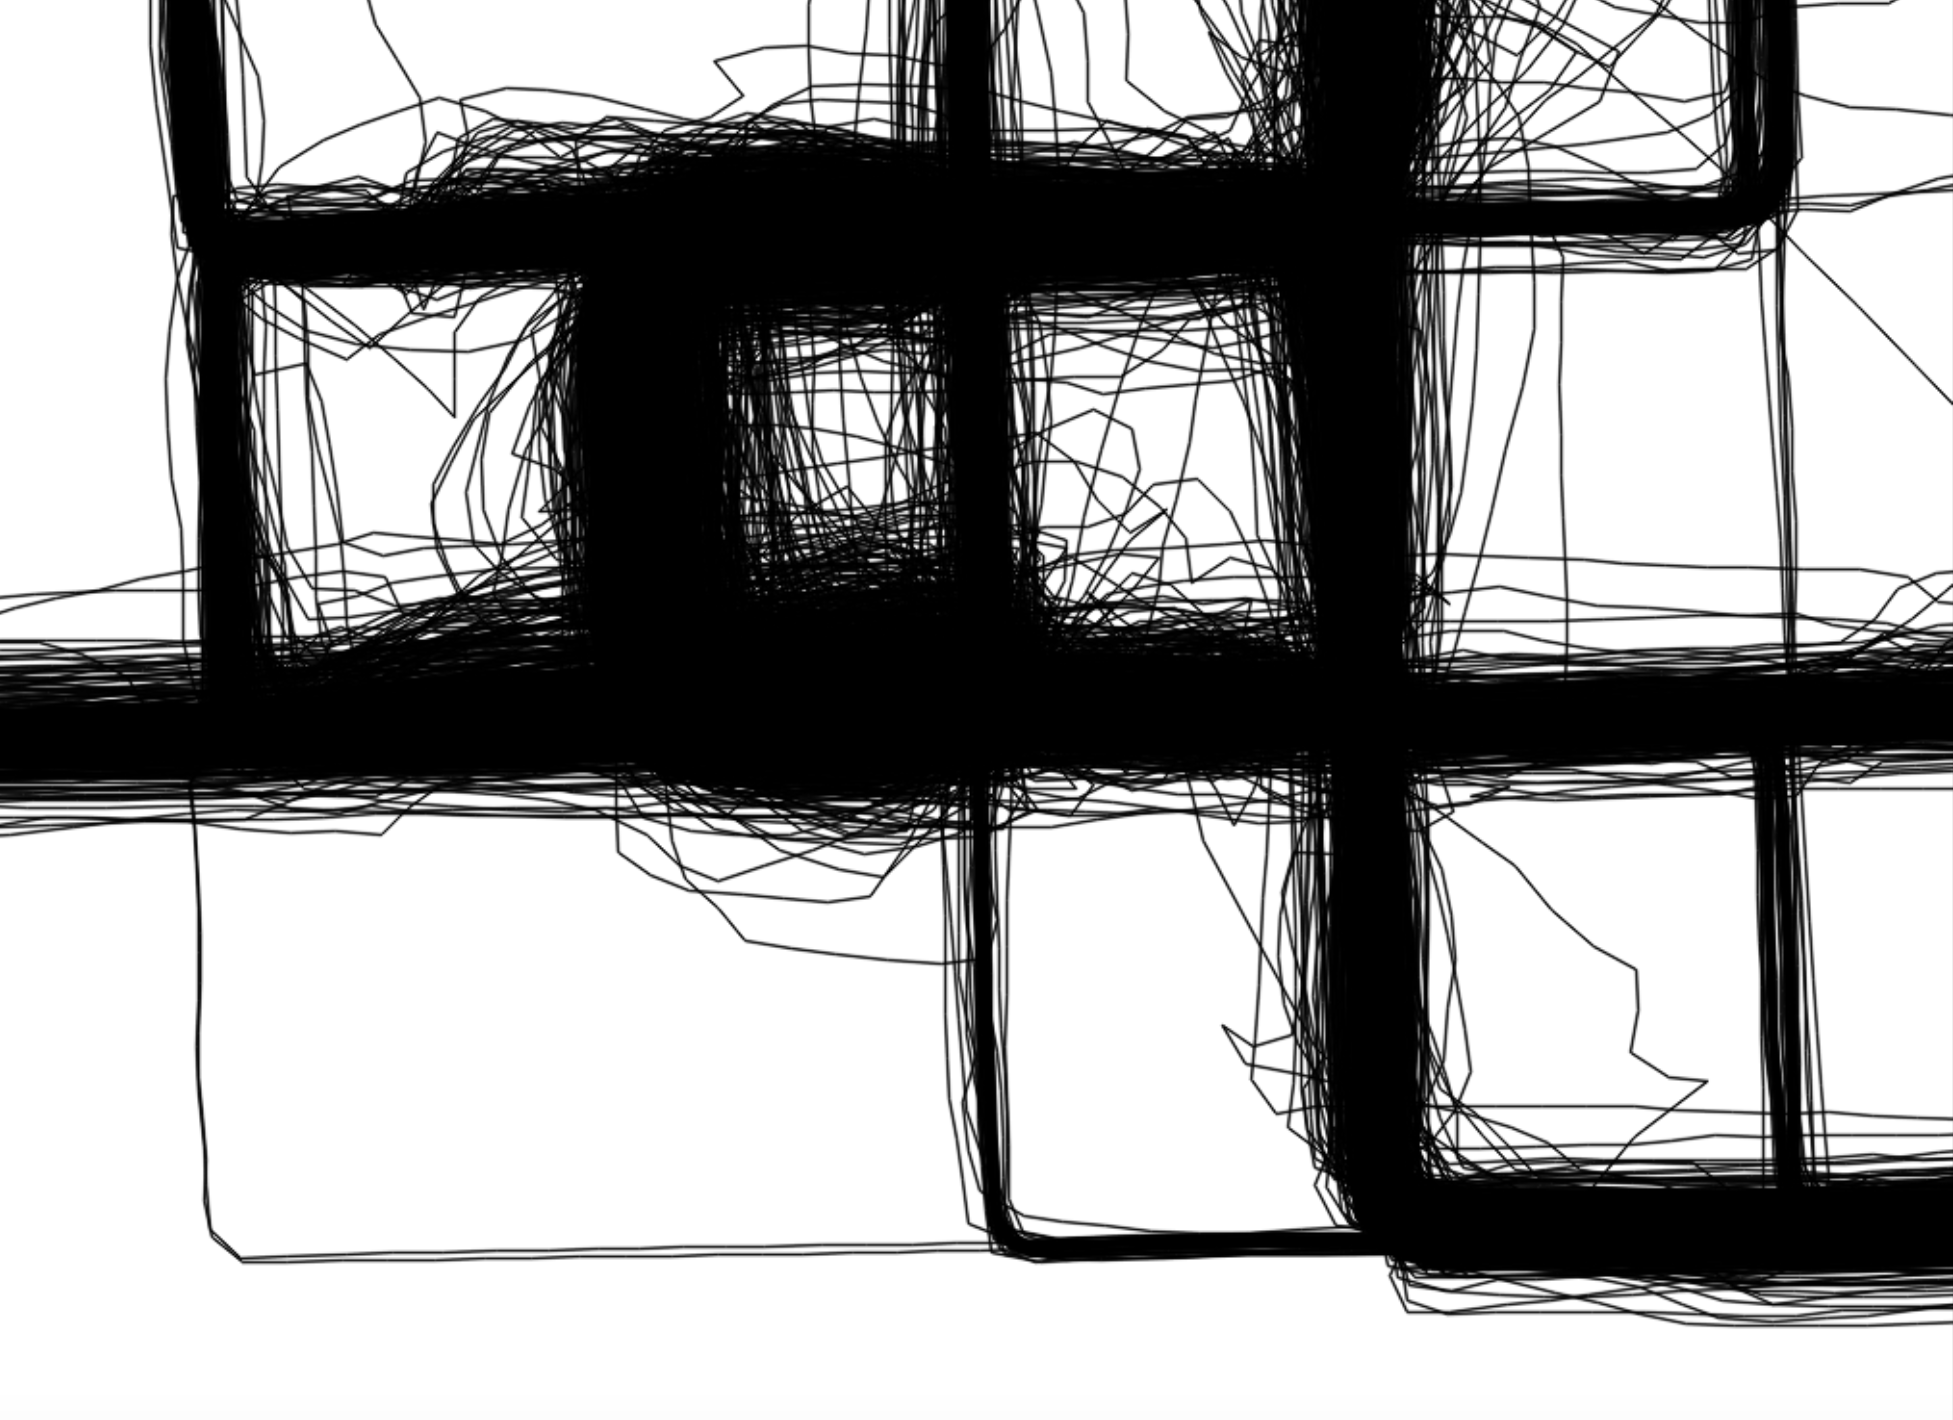
\includegraphics[width=0.5\linewidth]{Figures/Method/binmask.png}\label{fig:method/binmask} }}%   
 \subfloat[\textit{Kernel density estimate where more frequently travel roads are darker.}]{{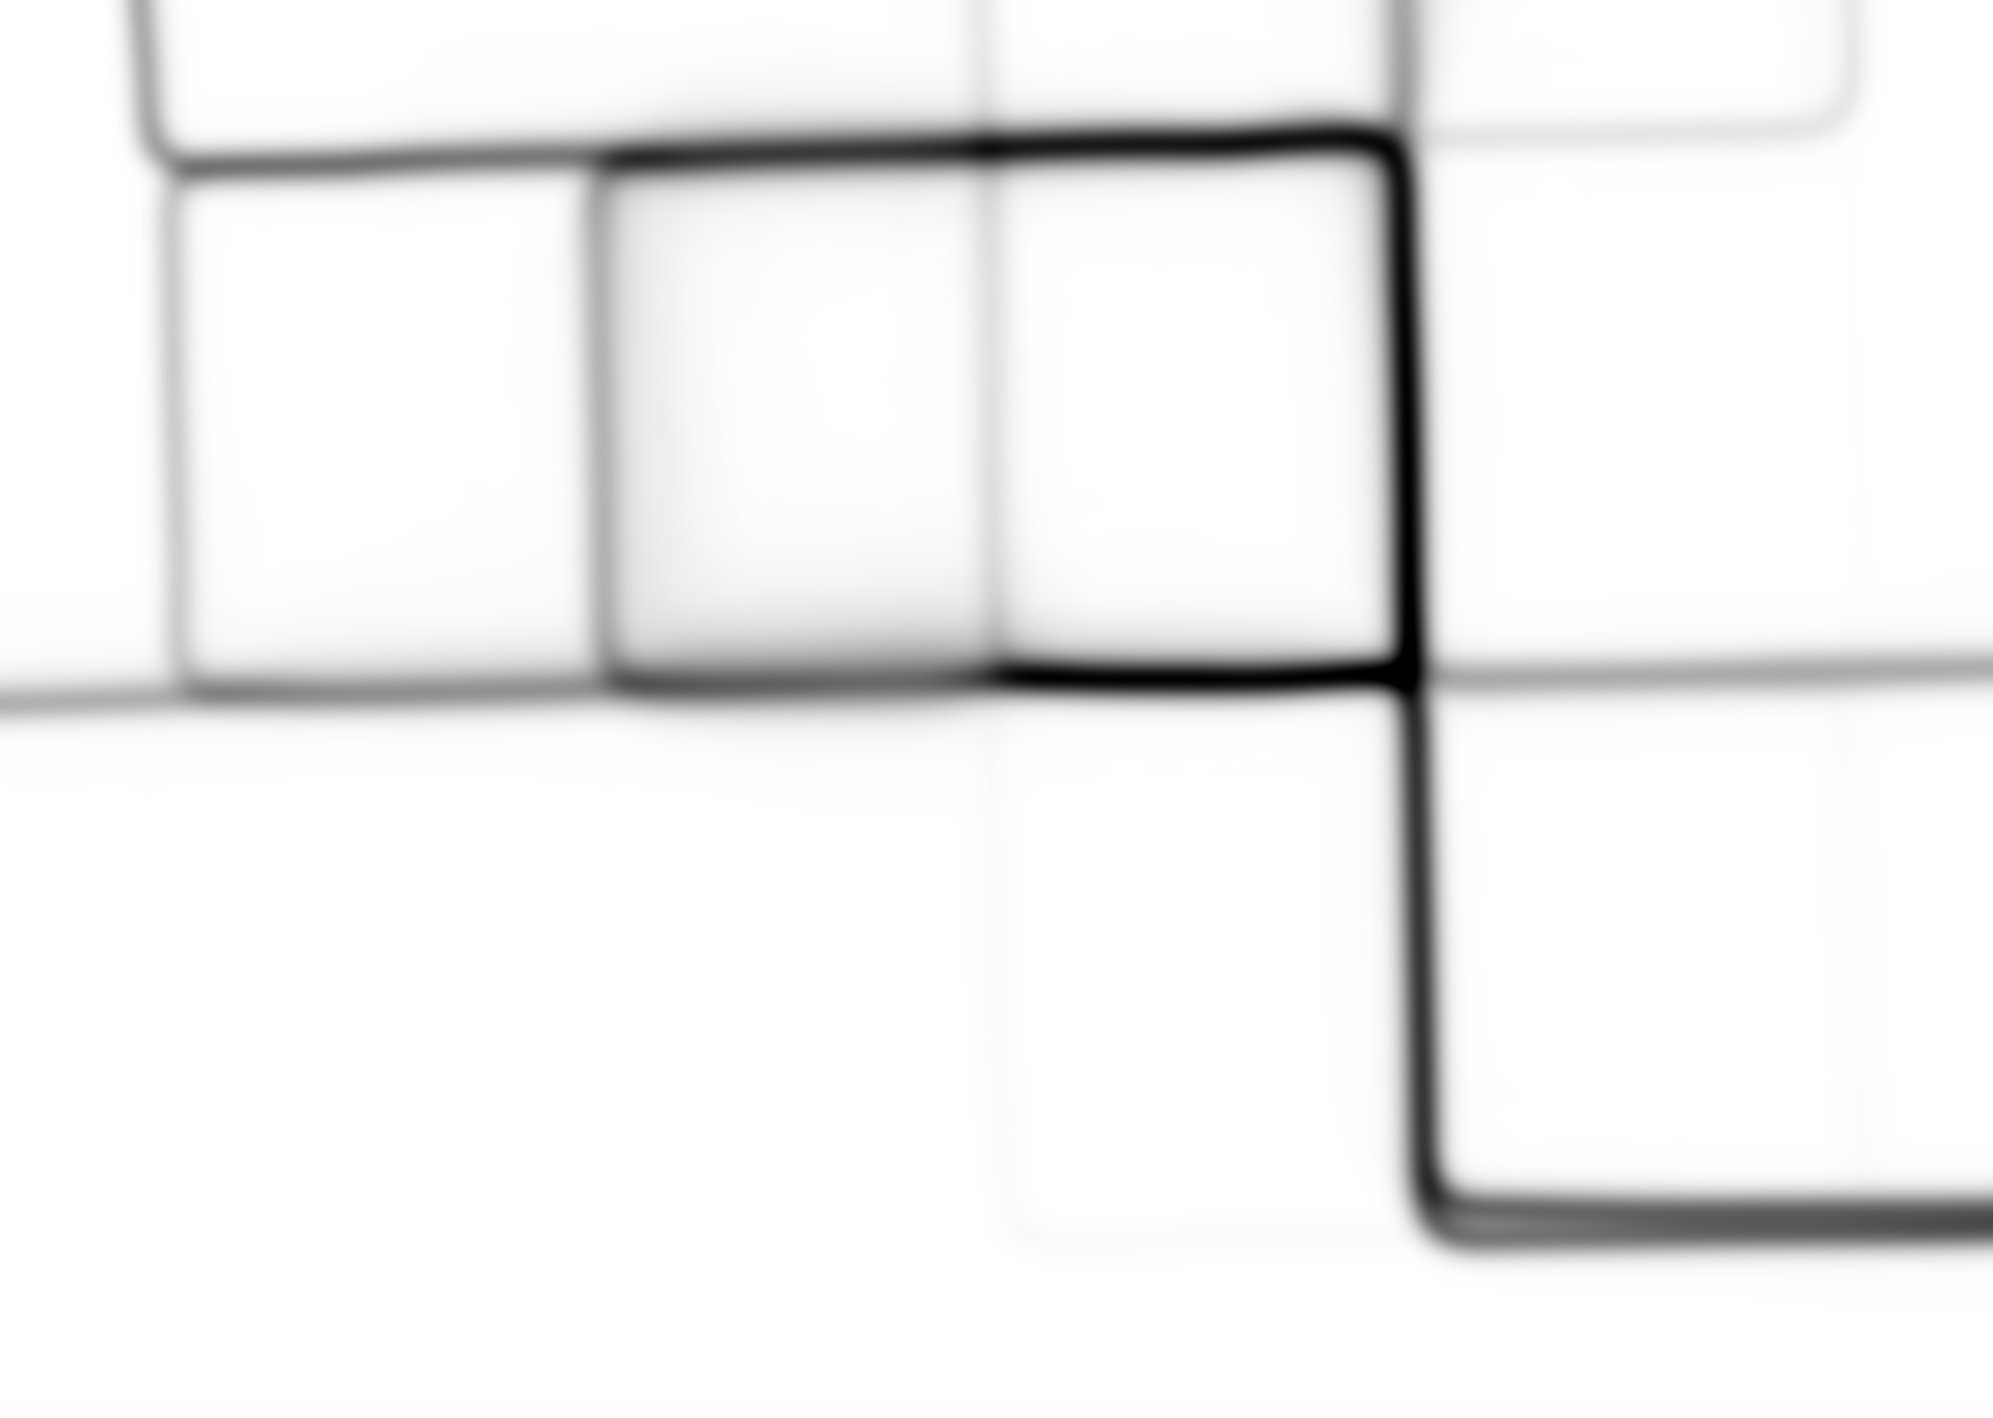
\includegraphics[width=0.5\linewidth]{Figures/Method/kdetraj.png}\label{fig:method/kde} }}%
 \caption{The density estimation creates a continuous distribution of the road network. Note that the noisy areas are quite faint. Illustration from \citep{biagioni:gis12}.}%
 \label{fig:method/binmaskkde}
\end{figure}

%------------------------------------------------------------------------%
\subsection{Initial map}
%------------------------------------------------------------------------%

\subsubsection{Gray-scale skeletonization}

Next, the aim is to extract road centerlines given the initial density estimate of the road network. \cite{biagioni:gis12} present a gray-scale skeletonization algorithm that for each integer density level performs a binary skeletonization algorithm on the thresholded image as described in section \ref{chp:theory.sec:mapgen.sub:skeleton}. At each level edges are potentially added, but never removed. % Restriction in levels to powers of two is done, producing close to identical initial maps with an exponential improvement in execution time.

To illustrate the binary and the gray-scale skeletonization figure \ref{fig:method/skel_bin} and \ref{fig:method/skel_gray} are included below. 

\begin{figure}%
 \centering
 \subfloat[\textit{Binary skeletonization.}]{{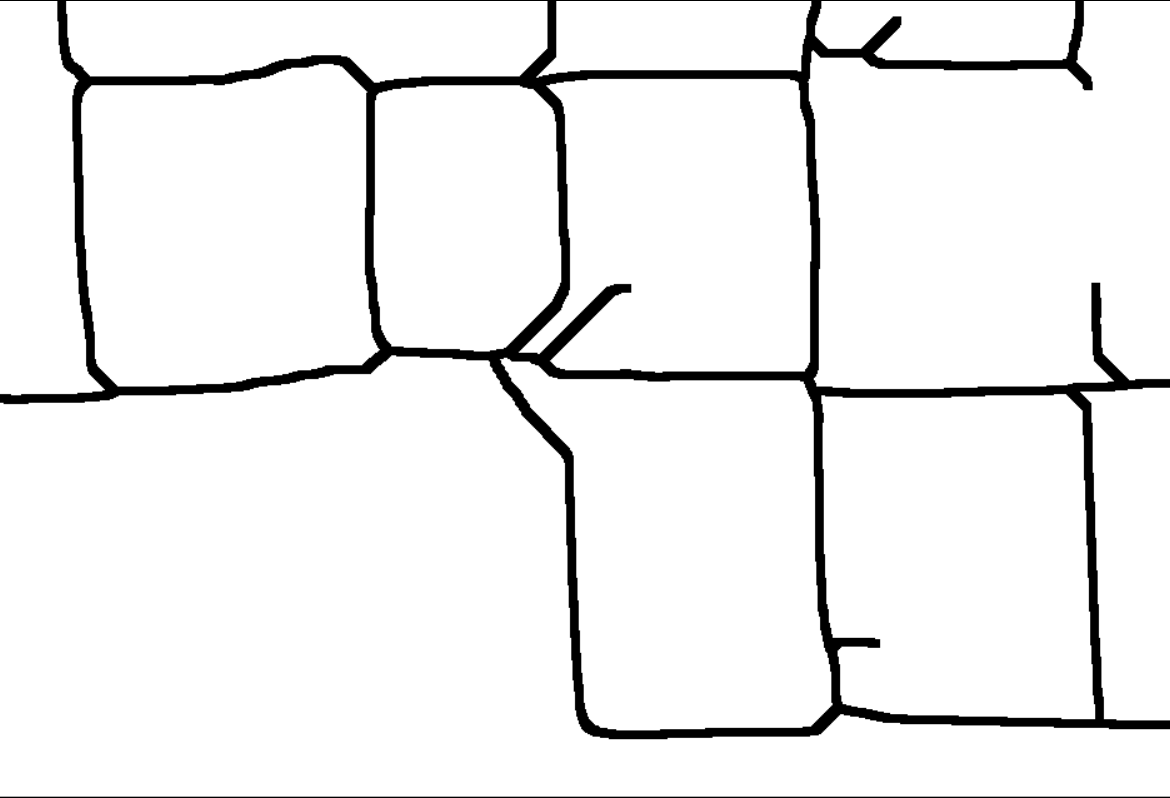
\includegraphics[width=0.5\linewidth]{Figures/Method/skel_bin.png}\label{fig:method/skel_bin} }}%   
 \subfloat[\textit{Gray-scale skeletonization.}]{{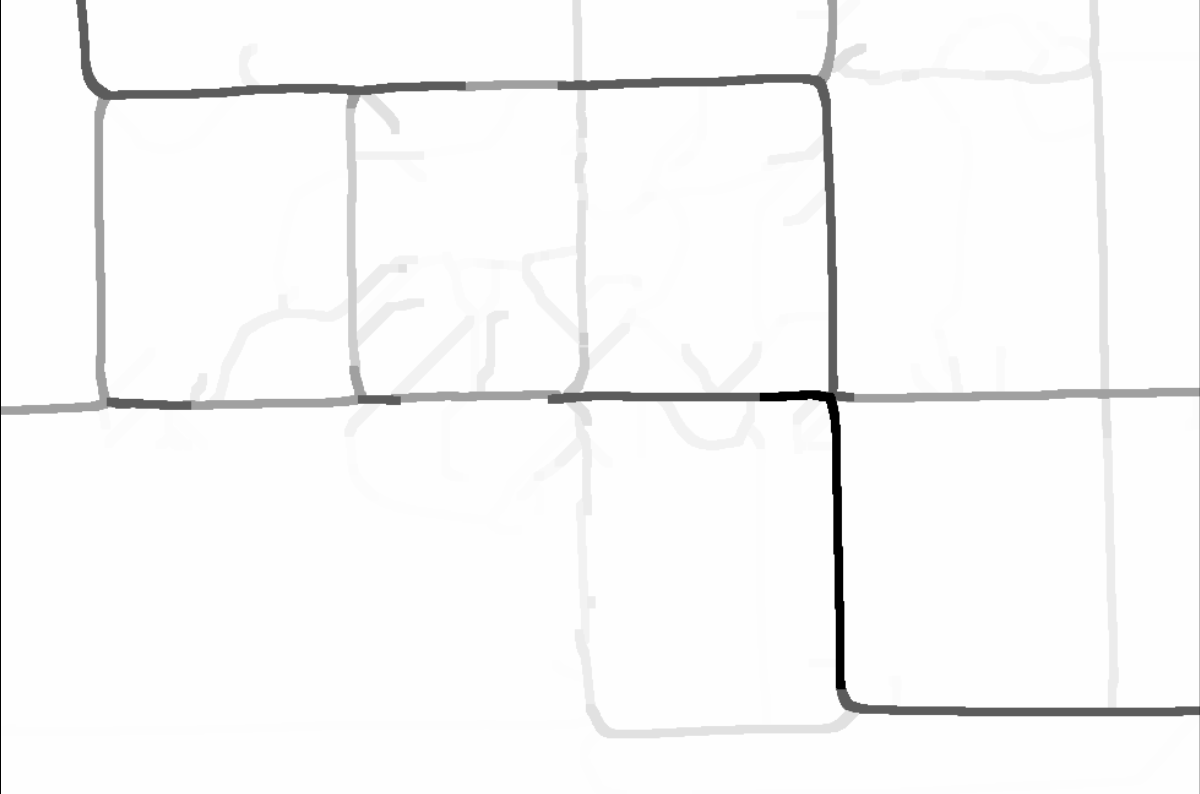
\includegraphics[width=0.5\linewidth]{Figures/Method/skel_gray.png}\label{fig:method/skel_gray} }}%
 \caption{The binary skeletonization thresholds only one integer density level whereas the gray-scale skeletonization produces several, creating more edges with associated confidence of location and existence. Illustration from \citep{biagioni:gis12}.}%
 \label{fig:method/skel}
\end{figure}

\subsubsection{Graph extraction from skeleton}

From the skeleton representation of the map a graph is to be extracted. The graph will be a representation of the road network where the intersections are nodes and the roads are edges. The edges in the graph will from now on be denoted as segments, furthermore these will be divided into edges. Hence, a segment is a road from one intersection to another and consists of one or several edges. 

To extract the graph from the skeleton an extended combustion technique proposed by \cite{21inBiagioni} is used. The technique is explained in more detail in section \ref{chp:theory.sec:mapgen.sub:comb}. Initially every crossing in the road network skeleton is found. By starting at a neighbouring pixel of a crossing the algorithm continuous walking on the segment until another crossing is detected by following a couple of given rules. This is done for all neighbours of all crossings. All segments are then extracted along with the crossings i.e. all pixels that have been associated with an edge. Hence the graph representation of the road network has been obtained. 

Finally the Douglas-Puecker algorithm, see section \ref{chp:theory.sec:dp}, is used to divide the segment up into edges, shaping the road segment. The algorithm finds, given a segment with a certain number of points, a similar curve with fewer points \citep{kondaveeti:clusters}. This set of fewer point are start- and end-points of the edges. Now the initial map has been obtained.

% examples of how the comb. tech. works. - drawings in hand written notes

%------------------------------------------------------------------------%
\subsection{Map matching to initial map}
%------------------------------------------------------------------------%
The trajectories, the observations, will now be matched to the initial map. Firstly a speed limit is enforced by dividing every edge in every segment into several fix-length states. Every state must be passed through before transition is made to the next state.

The graph is then used to create an \ac{HMM} representation of the road network. The transition probabilities are assigned the values of the edge weights in the graph. They are thereafter normalised having the total probability of 1 transferring to another state or stay in the current state. Furthermore the Viterbi algorithm is used for the actual map matching. 

%------------------------------------------------------------------------%
\subsection{Refining topology in the map}
%------------------------------------------------------------------------%

The initial map is refined by using the map-matched traces, see table \ref{tab:def}. First, spurious edges will be pruned. This is done by removing all edges with less than two well-matched traversals. It is performed using the following methodology. Let a trace $t$ consist of several traversals. Let $\tau$ be a traversal of an edge $e$ and $p \in \tau$ be its GPS points. For a traversal to be considered as well-matched to an edge $e$ the distance measure

% traversal = en edge har passerats. ett par påå varandra följande gps-punkter som matchats till samma är en traversal
% gps-puntker som matchats till en edge . . . . | * * * * , 
% . = gps-punkter med en label, * = gps-punkter med annan label

\begin{equation}
    \operatorname{RMSD}(\tau, e) = \sqrt{\frac{1}{|\tau|}\sum_{p \in \tau}{\operatorname{dist}(p, e)^2}}
\end{equation}

% abs av mängd är dess kardinalitet (antal element)
% t är index för traversal tau

must fulfil $\operatorname{RMSD}(\tau, e) < {RMSD}_{max}$ for a given value $RMSD_{max}$. For each trace $t$ and edge $e$ the number of well-matched traversals is denoted $n_e^t$. By considering all traces, the number of well-matched traversals to an edge $e$, $n_e = \sum_t{n_e^t}$, is found. If $n_e$ is less than two the edge $e$ is removed. Having $n_e$ = 0 is unlikely to represent a road and $n_e$ = 1 could have been created by a single traversal and should hence be considered spurious. % last sentence could be removed here 

The proposed algorithm to create a map doesn't always capture topology correctly, especially at positions with uneven density distribution such as intersections. Therefore, in ascending order, segments are collapsed into intersections which effectively modifies the map to be more accurate. A check is performed to see that all traces previously mapped to the segment are still well-matched, otherwise the change is reversed.

After this step traces are map matched again, this time using the number of traversals of each segment as transition probabilities.



% The traces of observations are modified by removing observations in observation blackout windows and also those that are too far from its matched edge (spurious). New edge weights are calculated based on the number of observations of each segment.

% Finally a refinement of the map is done. For each segment shorter than a fixed length it is collapsed into one node at equal distance from the head and tail node of the segment. If traces are still well matched after the change the node is kept and the segment deleted.

% After this step traces are map matched again, this time using the number of traversals of each segment as transition probabilities.


%========================================================================%
\section{Our contributions to map generation}
\label{chp:method.sec:contr_mapgen}
%========================================================================%

The code from \cite{biagioni:gis12} is open source and can be found at \citep{chicago}. This code however is written in Python 2 using OpenCV 2. Since Zenuity primarily uses Python 3 (and OpenCV 3) we therefore chose to convert the code. Initially the task was just to make the ``2-versions'' work since many packages and routines have been removed since the code was written back in 2012. Also minor modifications were made. The computational load between the ``2-versions'' and the ``3-versions'' was furthermore significantly decreased. This had to do with, for example, using numpy instead of OpenCV when handling matrices. 

Apart from the code conversion and the minor changes in the code we also added time stamps for each edge. More specifically, we map matched observations to edges and found the last observation that was matched to an edge and called it the \textit{time stamp} of that edge.
% Grundidé kommer härifrån, här tar vi ett steg bort... t ex timestamps på edges, indexering efter när kartan skapades.


% The code from \cite{biagioni:gis12} is open source and can be found at \citep{chicago}. This code however is written in Python 2 using OpenCV 2. Since Zenuity primarily uses Python 3 (and OpenCV 3) we therefore chose to convert the code. This took about 3 weeks in total. Initially the task was just to make the ``2-versions'' work since many packages and routines has been removed since the code was written back in 2012. Also minor modifications were made. By going through the code we understood the theory behind the map generation method better and the run time between the ``2-versions'' and the ``3-versions'' was also significantly decreased. This had to do with, for example, using numpy instead of OpenCV when handling matrices. In retrospect it was definitely a good decision converting the code. 

\newpage
%========================================================================%
\section{Update maps}
%========================================================================%
\label{chp:method.sec:fuse}
% map conflation

Tikz for inferred map + inferred map ++ fuse maps --> new inferred map


To update an existing map using a set of \ac{GPS} trajectories, it is common to use a map matching algorithm to identify traces that remains unmatched. We consider these to be new roads. Then, a map generation algorithm is used to create roads from the traces. The new roads are finally linked to the existing map \citep{crowdatlas}\citep{cobweb}.

We chose a slightly different approach where a collection of new \ac{GPS} trajectories will always be used to create an inferred map. This map will then be fused together with another map, either another inferred map or a high-quality slowly updated map such as \ac{OSM} \cite{osm} or Google Maps \cite{googlemaps}. \cite{fuse} suggests such a method taking two maps as input, creating a fused map.

Given two directed graphs $\mathcal{G}_1$ and $\mathcal{G}_2$, representing the base map and the new map, we want to create a new fused map

\begin{equation}
    \mathcal{G}_f = f(\mathcal{G}_1, \mathcal{G}_2). 
\end{equation}

The fused map should contain the connectivity from both source maps using only few new edges to avoid spurious ones. 


Algorithm \ref{alg:mapfuse} displays the pseudo code for the map fuse algorithm. The function \textit{FindOutliers} generates a set of outliers. That is, a set of nodes in map $M_2$ that were at least $d_o$, outlier distance, meters from map $M_1$. Meaning, nodes in $M_2$ that have no correspondence in $M_1$ which we can consider to be part of new roads. Using these, a sub-graph $\textit{new_roads}$ is generated. Next, the outliers are sorted according to decreasing distance from map $M_1$





\textbf{$d$ is used to find connections between new path and old map.}

% road addition procedure

\begin{algorithm}[H]
    \caption{MapFuse}
    \label{alg:mapfuse}
    \begin{algorithmic}
    \Function{MapFuse}{base road map $M_1$, inferred map $M_2$, matching distance $d_m$, outlier distance $d_o$} 
    
    \State $\textit{outliers} \gets \textsc{FindOutliers}(M_1, M_2, d_o)$
    \State $\textit{new\_roads} \gets \textsc{Subgraph}(M_2, \textit{outliers})$
    \For{$o \in \textit{outliers}$}
        \State compute $\textsc{distance}(o, M_1)$
    \EndFor
    \State $\textit{outliers} \gets \textsc{Sort}(\textit{outliers})$ \Comment{in decreasing order of distance to $M_1$}
    \For{$o \in \textit{outliers}$}
        \State $path \gets \textsc{BFS}(o, \textit{new\_roads})$
        \For{node $n \in path$}
            \If{$\textsc{distance}(n, M_1) \leq d_m$}
                \State $\textsc{merge}(n, argmin(n, M_1))$
            \EndIf
            \State $\textit{outliers} \gets \textit{outliers} - \{n\}$ \Comment{remove visited $\textit{outliers}$}
        \EndFor
    \EndFor
    
    \State \textbf{return} $M_1$
\EndFunction
\end{algorithmic}
\end{algorithm}



%------------------------------------------------------------------------%
\subsection{Add new roads to existing map}
%------------------------------------------------------------------------%


%------------------------------------------------------------------------%
\subsection{Delete roads}
%------------------------------------------------------------------------%
% and update weight

\textbf{anders artikel med konfidens??}
Tikz decision making flow chart


\subsection{Our contributions}

We add and delete edges based on time stamps and weights. Furthermore, we use several flags to understand which edges has been changed and how. 

\textbf{table with our flags?}


%========================================================================%
\section{Evaluation}
\label{chp:method.sec:evaluation}
%========================================================================%

To evaluate the inferred maps we need to compare them to some kind of ground truth. The goal of the map evaluation is to obtain a measure of similarity between maps, or more specifically, graphs. From the procedure described in section \ref{chp:method.sec:map} a graph is obtained that represents the road network and its connectivity. Further, a graph representing the ground-truth map, which we choose to be an \ac{OSM}, can be used for comparison. The \ac{OSM} can be obtained from \citep{osm} and is explained in further detail in section \ref{chp:data.sec:osm}.

As described in section \ref{chp:theory.sec:evaluation.sec:meth} there are many methods for comparing graphs. These methods focus mainly on topological similarities between graphs. Further, many existing map comparison algorithms focus mainly on geometrical similarities between roads, such as road length and orientation, and do not take connectivity into account \citep{ming}[\textbf{fler KÄLLor}]. In order to fully capture the similarities between maps we need a similarity measure that capture both the connectivity and geometry of the roads. Current state of the art for road network graph comparison can be divided into path based and set based methods.

Two different evaluation methods proposed by \cite{4inBiagioni} and \cite{biagioni:gis12} were implemented to both investigate the topological and geometrical similarities between the inferred and the ground-truth map. These two are set based. Further, a path based evaluation was done based on the method of \cite{pathbased}. To initially evaluate the accuracy of the generated map the \ac{OSM} will be used as ground truth. 

%------------------------------------------------------------------------%
\subsection{Geometry (GEO)}
\label{chp:method.sec:evaluation.sub:geom}
%------------------------------------------------------------------------%

A quantitative evaluation metric was proposed by \cite{biagioni:gis12} where the geometric accuracy of the inferred roads is evaluated. The idea is to place markers along each edge in the two maps with a fixed sample density, meaning that two consecutive markers will have a fixed distance between them. We then iterate through both sets of samples and try to find matching markers within the specified matching distance. We count all matched and unmatched markers in the inferred and base map and let

\begin{equation}
    \begin{split}
        precision &= \frac{\textit{matched\_inferred}}{\textit{matched\_inferred} + \textit{unmatched\_inferred}} \\ 
        recall &= \frac{\textit{matched\_base}}{\textit{matched\_base} + \textit{unmatched\_base}}.
\end{split}
\end{equation}

Further the F-score can be calculated according to equation \ref{eq:fscore}. Here, each marker can be matched to more than one other marker, that is we do not enforce a one-to-one matching between the two sets. Further no restriction is put on the allowed orientation difference between two matches. An illustration of the method can be seen in figure \ref{fig:method/comp_geo}.

\begin{figure}[H]
    \centering
    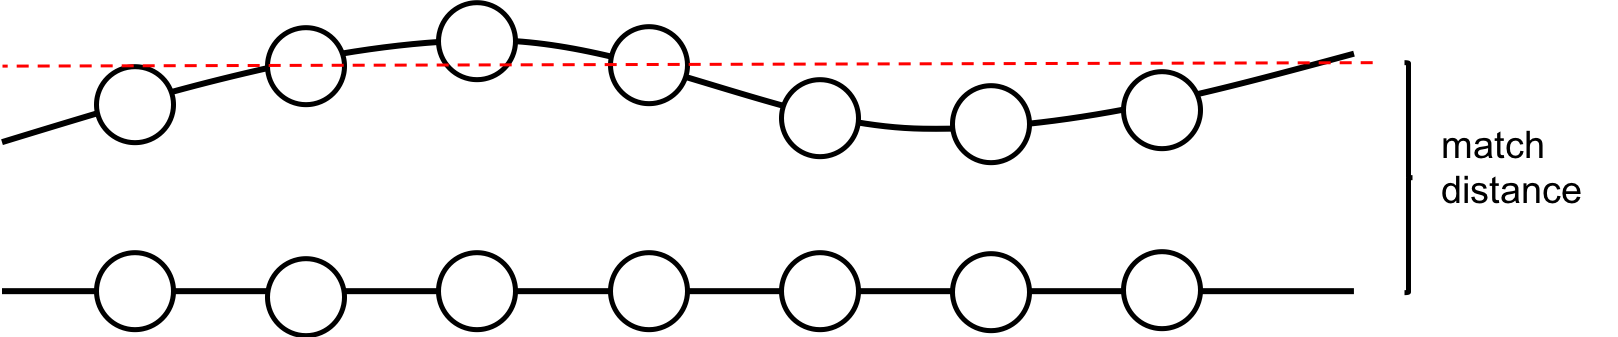
\includegraphics[width=10cm]{Figures/Method/geo.png}
    \caption{Illustration of the geometrical comparison.}
    \label{fig:method/comp_geo}
\end{figure}

% One deficiency with this method is the case when we infer a road that lies in between two close roads in the ground truth map. For this road, precision will be high while recall is low. 


%------------------------------------------------------------------------%
\subsection{Topology (TOPO)}
\label{chp:method.sec:evaluation.sub:topo}
%------------------------------------------------------------------------%

A method to evaluate both the topological and geometrical similarities between the road networks is further suggested by \cite{4inBiagioni}. The idea is to compare spatial samples in a local neighbourhood in each map. Starting from a random location in one map, edges are sampled outward at equal spacing until a maximum distance from the start point is reached. The closest corresponding location in the other map is found and the map is sampled locally out to the maximum distance. This allows for topology to be taken into account when comparing the maps. They let the samples taken in the ground truth map be known as \textit{holes} and samples in the inferred map as \textit{marbles}. Holes will then be filled with marbles if they are within a maximum matching distance and the difference in bearing is less than 45$\degree$. Each hole can be filled with at most one marble. Spurious edges, or possible new roads, will then correspond to unmatched marbles and missing roads in the inferred map will correspond to empty holes. 

Define the fractions

\begin{equation}
\begin{split}
        spurious &= \frac{\textit{unmatched\_marbles}}{\textit{unmatched\_marbles} + \textit{matched\_marbles}} \\ 
        missing &= \frac{\textit{empty\_holes}}{\textit{empty\_holes} + \textit{filled\_holes}}.
\end{split}
\end{equation}

The precision and recall of the inferred map can then be defined as

\begin{equation}
    precision = 1 - spurious, \quad recall = 1 - missing
\end{equation}

Further the F-score is calculated according to equation \ref{eq:fscore}. Figure \ref{fig:method/topo} displays an illustration of the method. In \ref{fig:method/a} holes have been dropped in the ground truth map and in \ref{fig:method/b} marbles have been dropped in the generated map. In \ref{fig:method/c} the holes are being filled by the marbles where the two maps overlap.


\begin{figure}[H]%
 \centering
 
 \subfloat[\textit{}]{{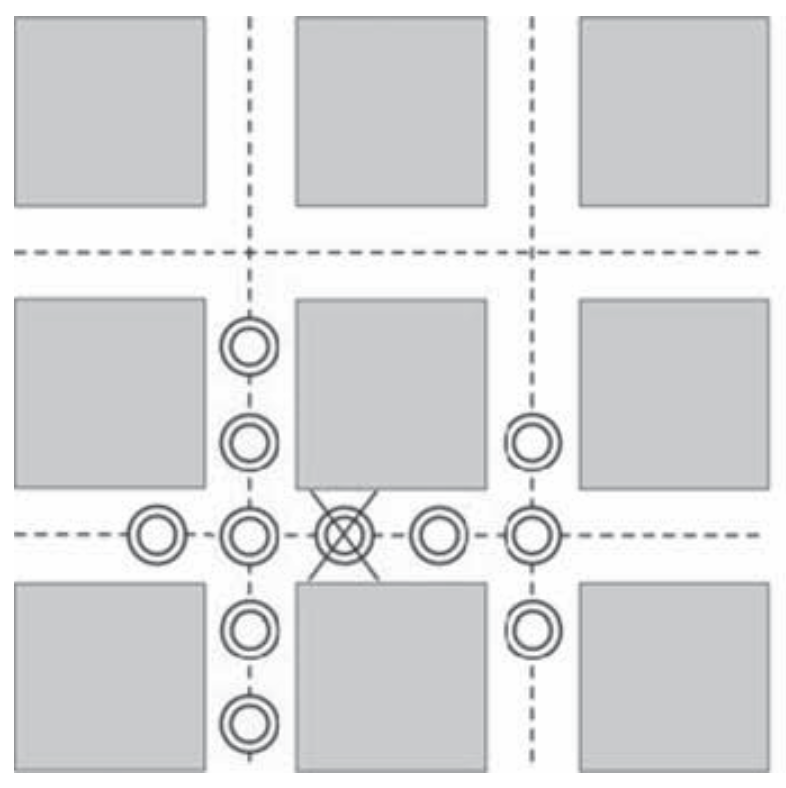
\includegraphics[width=0.33\linewidth]{Figures/Method/topoa.png}
 \label{fig:method/a} }}% 
 \subfloat[\textit{}]{{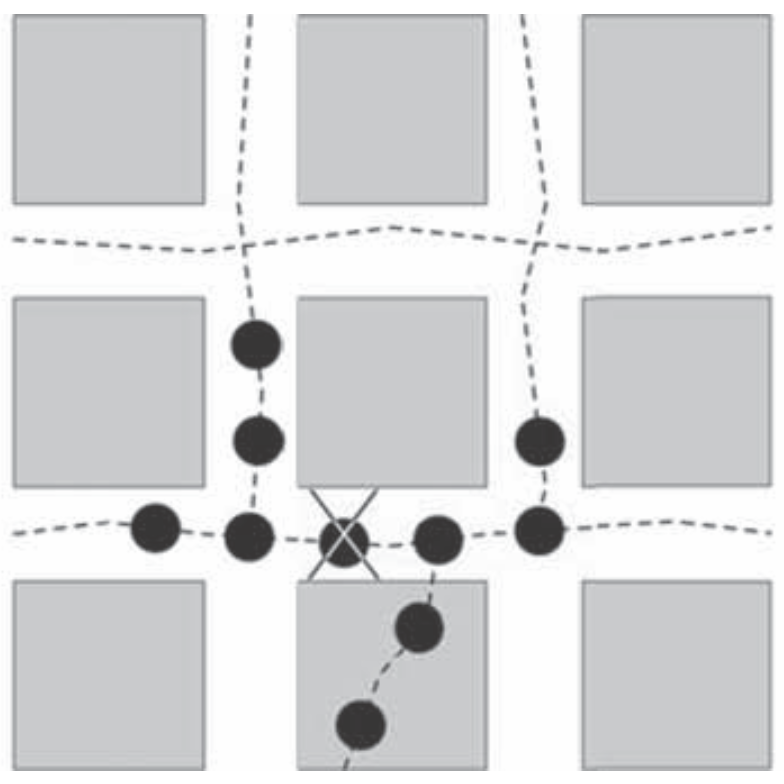
\includegraphics[width=0.33\linewidth]{Figures/Method/topob.png}
 \label{fig:method/b} }}%
 \subfloat[\textit{}]{{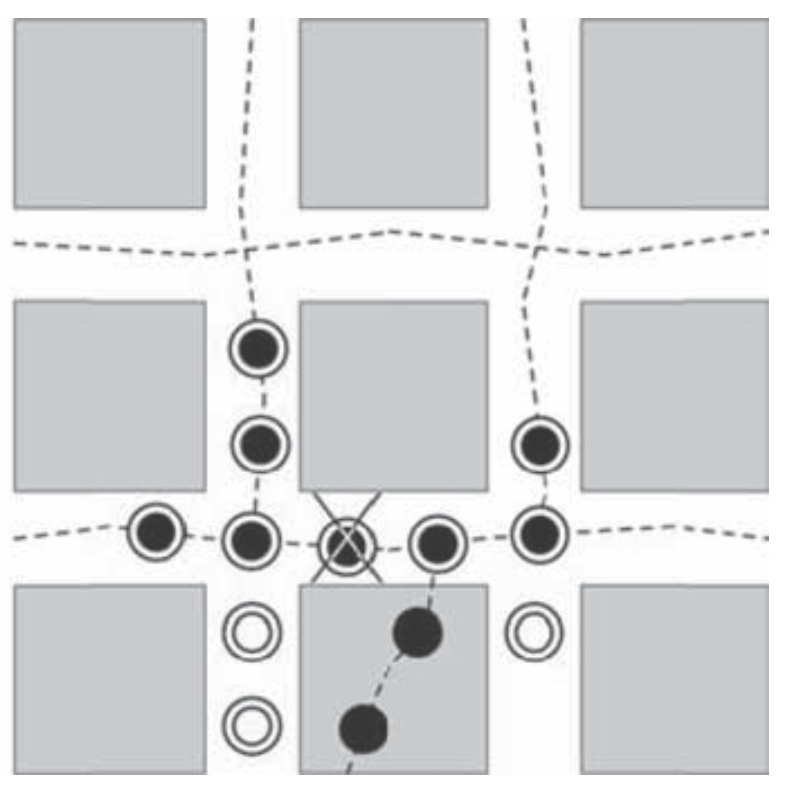
\includegraphics[width=0.33\linewidth]{Figures/Method/topoc.png}
 \label{fig:method/c} }}%
 
 \caption{Overview of map comparison algorithm: (a) holes dropped at fixed intervals (ground truth map), (b) marbles dropped at fixed intervals (generated map), and (c) marbles fill holes where maps overlap \citep{4inBiagioni}.}%
 \label{fig:method/topo}
\end{figure}

By using this local sampling technique we can obtain a measure of how similar the maps are as observed by each individual edge. For each edge we sample once locally first from the in node and then from the out node and calculate the F-score for each respective starting point. We then calculate the \textit{local signature}, $\Delta_e$, of an edge as the mean of the obtained F-scores. This value will be a measure of how similar the neighbourhood around an edge is in the two maps.


%------------------------------------------------------------------------%
\subsection{Path-based}
\label{chp:method.sec:evaluation.sub:pathbased}
%------------------------------------------------------------------------%
--->Our distance measure between two embedded graphs are based on the Fréchet distance between two paths.<---



Both the geometrical and topological method are based around the idea of comparing point sets induced by the graphs. \cite{pathbased} suggest an evaluation method based on similarities between coherent travel paths in the graphs. Each graph will be represented by a set of paths of varying length. As a distance measure for comparing the graphs they calculate the directed Hausdorff distance between path sets, defined in equation \ref{eq:dhausdorff} in section \ref{chp:theory.sec:evaluation.sub:stat.sub:dist}. The Fréchet distance, see equation \ref{eq:frechet} in section \ref{chp:theory.sec:evaluation.sub:stat.sub:dist}, will be used to compute the distance between two paths, letting the underlying distance metric $d$ be the Euclidean norm. 

Let $G$ and $H$ be two graphs and $\Pi_G, \Pi_H$ be the set of all paths in each graph. Then for $\pi_G\subseteq\Pi_G, \pi_H\subseteq\Pi_H$ a formal definition of the \textbf{directed} path based distance is given as

\begin{equation}
    \overrightarrow{d}_{path} (\pi_G, \pi_H) = \max_{p_G\in \pi_G} \min_{p_H\in \pi_H} \delta_F(p_G, p_H)
\end{equation}

where $\delta_F$ is the Fréchet distance and $\overrightarrow{d}_{path}$ is the directed Hausdorff distance. Using link-length three paths, we let $\pi_G = \Pi_G^3$ and $\pi_H = \Pi_H$. That is, we iterate through all link-length three paths in the ground-truth map, $G$, and find the closest matching path of arbitrary link-length in the inferred map, $H$. % Given that there are $| \Pi_G^3 | \in O(m^3)$ paths of link-length 3 in graph $G$, where $m$ is the total number of nodes and edges, $\overrightarrow{d}_{path} (\Pi_G^3, \Pi_H)$ can be computed in polynomial time. 

Comparing all possible path sets is infeasible. However, \cite{pathbased} show that using link-length three paths they are able to approximate distances between paths of arbitrary length in polynomial time. The link-length is defined as the number of edges that the path contains. Note that they consider a link to be between intersection nodes, what we define as segments, such that link-length three paths better will capture driving routes in the two graphs.

The path-based distance measure returns a single value as a measure of similarity between graphs. To obtain more information on graph similarity we consider also the local signature of edges, defined for $e\in \mathcal{E}_G$ and $k \geq 1$ as $\Delta_{k,e} = \overrightarrow{d}_{path} (\Pi_e^k, \Pi_H)$. 

Can be parallelised to make run time decrease. (s. 16)

% pathbased s. 7 längst ner
Here we refer to figure \ref{fig:theory/path}.

\begin{figure}[H]
    \centering
    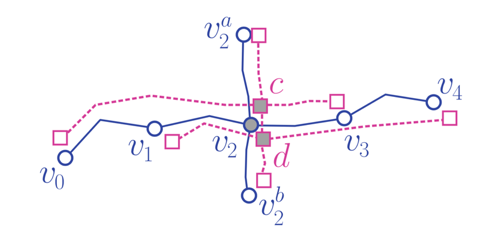
\includegraphics[width=10cm]{Figures/Method/path.png}
    \caption{Graph $H$ is shown in solid lines and graph $G$ in dashed lines. Link-length three paths in $H$ such as $v_0, v_1, v_2, v_3$ have corresponding paths in $G$. By performing \textbf{surgery} in these, a path in $G$ can be constructed that corresponds to the link-length four path $v_0, v_1, v_2, v_3, v_4$ in $H$ \citep{pathbased}.}
    \label{fig:theory/path}
\end{figure}


Code is open source and they want us to refer to:
Should you use the source code and/or data from this site, please cite also the following paper:

M. Ahmed, S. Karagiorgou, D. Pfoser, and C. Wenk. A Comparison and Evaluation of Map Construction Algorithms. GeoInformatica, 19(3):601-632, 2015.

DOI: 10.1007/s10707-014-0222-6 - paper


The numbers in the colour bar corresponds to the local edge signatures explained in \ref{chp:method.sec:evaluation.sub:pathbased}.

We will later denote the \textit{base map} being the map that is partitioned up into paths of different link length. In the other map corresponding paths will be found.

%========================================================================%
\section{Open source}
\label{chp:method.sec:opensource}
%========================================================================%

We have chosen to make the code public...





